\paragraph{UC-52 Visualizzazione stanze da igienizzare}
    \begin{itemize}
        \item \textbf{Attore primario:} igienizzatore;
        \item \textbf{Descrizione:} l’igienizzatore può visualizzare l'elenco delle stanze (contrassegnate dal nome univoco) da igienizzare;
        \item \textbf{Precondizione:} l'igienizzatore si trova nell’apposita sezione di visualizzazione delle stanze da igienizzare; 
        \item \textbf{Postcondizione:} l'igienizzatore ha ricevuto l'elenco delle stanze da igienizzare;
        \item \textbf{Scenario principale:} 
            \begin{enumerate}
                \item il sistema elabora la richiesta;
                \item il sistema restituisce la lista delle stanze da igienizzare.
            \end{enumerate}
    \end{itemize}
%TODO: controllare
\paragraph{UC-53 Marcatura stanza come igienizzata}

    \begin{itemize}
        \item \textbf{Attore primario:} igienizzatore;
        \item \textbf{Descrizione:} l’igienizzatore può marcare un'intera stanza come igienizzata, pertanto ogni postazione al suo interno è sanificata e servibile quindi dagli utenti. Tale azione viene certificata tramite la scansione del tag RFID associato alla stanza;
        \item \textbf{Precondizione:} l'igienizzatore naviga nell’apposita sezione di igienizzazione della stanza; 
        \item \textbf{Postcondizione:} l'igienizzatore ha marcato con successo una stanza come igienizzata;
        \item \textbf{Scenario principale:} 
            \begin{enumerate}
                \item l'igienizzatore seleziona la stanza da marcare come igienizzata;	
                \item l'igienizzatore contrassegna la stanza come igienizzata scansionando il tag RFID ad essa associata (UC-53.1 Scansione del tag RFID per segnalare la pulizia di una stanza);
                \item il sistema elabora correttamente la richiesta contrassegnando tutte le postazioni all'interno della stanza come igienizzate.
            \end{enumerate}
    \end{itemize}

\begin{figure}[H]
    \centering
        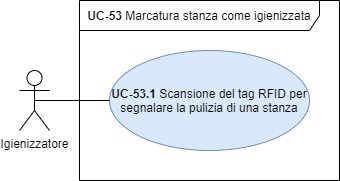
\includegraphics[scale=0.50]{src/CasiDUso/immagini/StanzaIgienizzata.png}
            \caption{Diagramma relativo alla pulizia di una stanza}
    \end{figure}
    

\paragraph{UC-53.1 Scansione del tag RFID per segnalare la pulizia di una stanza}

    \begin{itemize}
        \item \textbf{Attore primario:} igienizzatore;
        \item \textbf{Descrizione:} l’igienizzatore vuole scansionare il tag RFID della stanza per marcarla come igienizzata;
        \item \textbf{Precondizione:} l'igienizzatore ha selezionato la stanza da marcare come igienizzata; 
        \item \textbf{Postcondizione:} l'igienizzatore ha scansionato con successo il tag RFID;
        \item \textbf{Scenario principale:} 
            \begin{enumerate}	
                \item l'igienizzatore appoggia il proprio dispositivo sul tag della stanza igienizzata;
                \item il tag viene scansionato dall'applicazione;
                \item il sistema elabora la richiesta e contrassegna tutte le postazioni all'interno della stanza come igienizzate.
            \end{enumerate}
    \end{itemize}
